%\newpage\Large\mathphyssubsubsec{Lehramt Physik}\small
\section{Physik 50\% (Lehramt)} % oder: physik-Lehramt?

Der 50\%-Bachelorstudiengang Physik ersetzt ab dem Wintersemester 15/16 den Physik-Lehramtsstudiengang. Er hat einerseits die Aufgabe, die notwendigen fachlichen Kompetenzen für den Physikunterricht beizubringen und den Übergang zum Master of Education zu ermöglichen. Andererseits soll ein Übergang in den Physik-Masterstudiengang möglich sein. Es ist unausweichlich, dass der so entstehende Studiengang für keinen der beiden Wege die optimale Lösung darstellt. Dennoch versucht der Studiengang, diese Bedingungen irgendwie umzusetzen. Wie, wird im Folgenden vor diesem Hintergrund beschrieben.

\subsection{Fächerkombinationen}

Gemäß Prüfungsordnung darf der 50\%-Bachelor Physik mit allen anderen 50\%-Studiengängen an der Universität Heidelberg, die für einen Master of Education qualifizieren, kombiniert werden. Unabhängig von der Fächerkombination darf am Ende dieses Studiums die Bachelorarbeit in Physik geschrieben werden, sie muss aber nicht. Man kann sein erstes Hauptfach, in dem die Bachelorarbeit geschrieben wird, auch unkompliziert im Laufe seines Studiums tauschen. Allerdings ist die Kombination mit Mathematik zu empfehlen, da nur so mathematische Grundlagen erworben werden können (siehe dazu den Abschnitt „Mathematische Grundlagen“) und mit der Mathematik die Überschneidungsfreiheit von Pflichtveranstaltungen noch am besten gewährleistet ist.

\subsection{Arbeitspensum}

Wie erwähnt muss der 50\%-Bachelor Physik auch für den Physik-Master qualifizieren. Dies heißt, dass die grundlegenden Vorlesungen „Experimentalphysik“ 1-5 (\gls{Ex}) und „Theoretische Physik“ 1-4 (\gls{Theo})\footnote{Die Abkürzung „Theo“ kann zu Verwirrungen mit Informatikern führen, da diese das als „Theoretische Informatik“ verstehen.} verpflichtend vorgeschrieben und in den ersten fünf, bzw. vier Semestern gehört werden müssen. Dies führt besonders in den ersten beiden Semestern zu einem hohen Arbeitspensum: Ist das zweite Fach beispielsweise Mathematik, so müssten im ersten Semester im Prinzip die Vorlesungen Ex 1, Theo 1, „Analysis 1“ (\gls{Ana}) und „Lineare Algebra 1“ (\gls{LA}) gehört werden. Zum Vergleich: Für den 100\%-Bachelor Physik sieht die Fakultät drei Vorlesungen dieses Umfangs pro Semester als angemessen an.

Wir empfehlen daher, sich im ersten Semester auf diese drei Vorlesungen zu konzentrieren und den Theoriezyklus ein Jahr später, im dritten Semester, beginnen zu lassen. Somit fällt die Theo 4 zwar in das sechste Semester, es ist unter 50\%-Studierenden jedoch sowieso sehr unüblich, dass sie bereits im sechsten Semester ihre Bachelorarbeit schreiben. Obwohl die Theo 1 auch für Experimentalphysik relevante mathematische Methoden beinhaltet ist ihr nach Hintenschieben der Experimentalphysik 1 vorzuziehen, da letztere die Orientierungsprüfung ist, die bis zum dritten Semester bestanden werden muss. Ein Großteil der Arbeit ist auf die Vorlesungszeit konzentriert, während in der vorlesungsfreien Zeit (abgesehen von Labor- und Schulpraktika) nicht viel geschieht. Das erste Schulpraktikum, das sogenannte Berufsorientierende Praktikum (BOP 1) kann man auch direkt in den ersten Semesterferien absolvieren, wenn man sich rechtzeitig zu Beginn des ersten Semesters anmeldet.

Das 50\%-Studium mit Lehramtsoption ist noch weit entfernt davon, ausgereift zu sein, und viele Feinheiten hängen auch sehr vom Kombinationsfach ab, sodass man es als Lehramtsstudi leider nicht immer leicht hat. Wir als Fachschaft stehen euch dabei, neben anderen Anlaufstellen, soweit wie möglich als Ansprechperson zur Verfügung (siehe \autoref{lehramtkontakte}). Im Laufe des Vorkurs wird es auch ein spezielles 50\%lerinnen-Treffen zusammen mit einer 50\%-Studentin aus dem höheren Semester geben, sodass ihr bereits dort wichtige Tipps und Erfahrungen auf den Weg bekommt. 

\begin{figure*}[b]
\centering
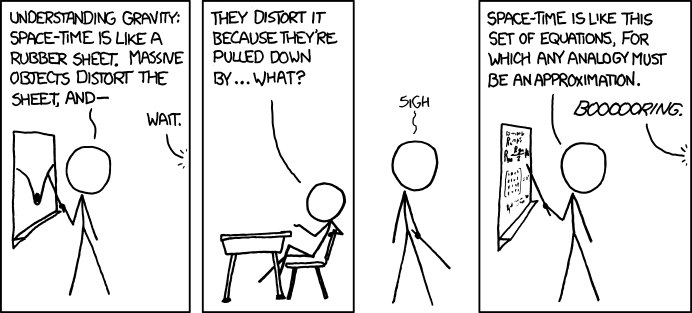
\includegraphics[width=\textwidth]{bilder/teaching_physics.jpg}
\end{figure*}


\subsection{Mathematische Grundlagen}

„Mathematik ist die Sprache der Physik“ -- heißt es so schön und ist in der Tat korrekt. Man könnte sogar weiter gehen und sagen, dass die Menschheit nur deshalb begonnen hat, Mathematik zu betreiben, weil sich damit die Natur beschreiben lässt. Dies heißt aber auch, dass alle, die Physik betreiben -- sei es an Schulen, Universitäten oder in der Wirtschaft -- ein Grundverständnis für Mathematik benötigen. Für diejenigen unter euch, die Mathematik als zweites Fach gewählt haben, ist das Folgende nicht relevant, da die dort vorgesehenen Mathematik-Vorlesungen sicher mehr als nur ein Grundverständnis für Mathematik beibringen. 

Vieles der Mathematik, die in den ersten Semestern gebraucht wird, wird in den Physik-Vorlesungen behandelt. Grund dafür ist, dass die Fakultät für Mathematik und Informatik die Inhalte ihrer Vorlesungen natürlich an ihren eigenen Zielen und nicht denen des Physik-Studienganges ausrichtet. So beinhaltet beispielsweise die Vorlesung Theo 1 einen großen Mathematik-Teil, in dem beispielsweise die Lösung von Differentialgleichungen behandelt wird.

Allerdings sind nicht ohne Grund für den 100\%-Bachelorstudiengang Physik die Vorlesungen LA 1 sowie wahlweise „Höhere Mathematik für Physiker“ 2 und 3 (\gls{HoMa}) oder Ana 2 und 3 vorgeschrieben. Zum Beispiel ist die theoretische Beschreibung der Quantenmechanik ohne Kenntnis über Eigenvektoren aus LA 1 nicht zu verstehen. Das Beste wäre also, wenn all jene, die nicht Mathematik als zweites Fach gewählt haben, zumindest LA 1 vor Theo 4 hören (oder ein Buch lesen) würden. Diese Vorlesungen sind im Modellstudienplan allerdings nicht vorgesehen, wodurch dies quasi freiwillige Zusatzarbeit wäre, da das 50\%-Studium keinerlei Spielraum für zusätzliche Leistungspunkte aus Wahlfächern vorsieht.


